
%%%%%%%%%%%%%%%%%%%%%%%%%%%%%%%%%%%%%%%%%%%%%%%%%%%%%%%%%%%%%%%%%%%%
\setcounter{section}{1}
\begin{center}
\section*{Введение}
\addcontentsline{toc}{section}{Введение}
\end{center}

Фильмы привлекают миллионы зрителей. Фильмы - это не просто развлечение, мы получаем что-то более глубокое из кинокартин, которые мы смотрим. Просмотр также может быть способом оценить искусство в формате, более доступном для многих из нас, чем посещение музея. Кино также позволяет нам извлечь некоторые уроки, опираясь на опыт героев. Я решил сделать мобильное приложение на тему информационно-справочная система «Фильмотека домашняя», потому что, я люблю смотреть фильмы и для меня эта тема очень интересна. Хоть и на сегодняшний день уже существуют, очень много подобных приложений, и все же я хочу попробовать сделать что-то свое. Да и к тому же в ходе создания данного приложения, я смогу получить очень много полезных знаний в среде мобильной разработки. 

\noindent В данной курсовой работе нам предстоит сделать:	
\begin{itemize}
\item Cоздать ядро OС (операционной системы) Linux.
\item Подключить модули, которые потребуются для нашего приложения.
\item Создать дизайн приложения.
\end{itemize}

\noindent Структура курсовой работы состоит: 
\begin{itemize}
\item Введение (Общая характеристика курсовой работы)
\end{itemize}
\begin{itemize}
\item Основная часть (Выполнение заданий данных в этой курсовой работе)
\end{itemize}
\begin{itemize}
\item Заключение (Результаты и итоги курсовой работы) 
\end{itemize}
\begin{itemize}
\item Источники (Ресурсы использованные в ходе выполнения курсовой работы)
\end{itemize}

\subsection{Анализ предметной области}

Как уже было выше сказано, фильмы это не только развлекательный, но и полезный контент, который интересен очень многим людям разной возрастной категории. Поэтому нужно сделать дизайн своего приложения простым и приятным на вид людям. Таким образом наше приложение на тему информационно-справочная система «Фильмотека домашняя» сможет получить широкое распространение среди любителей фильмов и простых, удобных приложений.

%%%%%%%%%%%%%%%%%%%%%%%%%%%%%%%%%%%%%%%%%%%%%%%%%%%%%%%%%%%%%%%%%%%%

\setcounter{subsection}{0}
\begin{center}
\section*{Основная часть}
\addcontentsline{toc}{section}{Основная часть}
\end{center}
\subsection{Ядро OC Linux}
Ядро — это самая привилегированная программа на компьютере. Если говорить конкретно о ядре Linux, то оно монолитное. Иными словами, в режиме ядра работает всё необходимое для управления ресурсами компьютера. В пользовательском режиме также имеются программы для управления, но они лишь расширяют возможности ядра.

Задача ядра – общаться с аппаратным и программным обеспечением и максимально эффективно управлять ресурсами системы. Оно взаимодействует с оборудованием через драйверы, которые включены в ядро. К примеру, когда приложение хочет что-то сделать скажем, изменить настройку громкости динамиков, оно может просто отправить этот запрос ядру, и ядро может использовать драйвер для динамиков, чтобы фактически изменить громкость.

Практически каждое обновление ядра будет иметь какие-то исправления безопасности, которые закрывают обнаруженные дыры. Это, вероятно, одна из самых важных причин для обновления вашего ядра, так как вам всегда будет безопаснее с исправленным ядром. 
Обновления ядра содержат не только исправления безопасности, но и другие проблемы, которые могут вызвать сбой системы при регулярном использовании. Также обновленное ядро может включать в себя новые функции ядра и последние версии драйверов, что может улучшить скорость работы системы.

Несмторя на столько плюсов, в современных реалиях увеличение производительности при сборке ядра совсем незаметно. Сейчас сборка ядра может понадобиться пользователям не бинарных дистрибутивов, таких как\newline Gentoo, тем, кто хочет внести некоторые изменения в ядро, получить новую  версию ядра и, конечно, же тем, кто хочет полностью разобраться в работе своей системы.

В этой курсовой работе мы рассмотрим как собрать ядро Linux на примере дистрибутива Ubuntu. Это можно сделать вручную или же в автоматическом режиме. Так как ручной процесс сборки сложный и не быстрый, я буду это делать в автоматическом режиме.

%  \begin{\normalsize}
    \subsubsection{Создание виртуальной машины в Oracle VirtualBox}
%   \end{\normalsize}
Сперва создадим виртуальную машину Ubuntu Linux., где мы будем собирать ядро. Для этого я буду использовать VirtualBox, так как в нем создать виртуальную машину очень просто, к тому же я это уже делал на практических занятиях несколько раз. 

\image{vbbox.png}{Официальный сайт VirtualBox}
\newpage
После установки мы скачиваем дистрибутив операционной системы Ubuntu Linux. Можно было выбрать и другой дистрибутив, но мне приятнее работать в Ubuntu. 

\image{ubuntu.png}{Сайт русскоязычного сообщества Ubuntu}

После заходим в VirtualBox. Далее нажимаем создать. В первом окне вводится имя виртуальной машины, а также тип ОС которая будет запущена на ней. В следующих шагах создания виртуальной машины надо выбрать объём оперативной памяти, размер жёсткого диска, формат хранения файлов жёсткого диска. После в левом столбце можно заметить созданную виртуальную машину.

\image{p1.png}{Cоздание виртуальной машины}
\newpage
Характеристики моей виртуальной машины.
\image{p2.png}{Характеристики вирутальной машины}
\newpage

После настройки параметров виртуальной машины нам нужно поставить образ Ubuntu. Для этого нажимаем настроить в верхней части экрана. В появившейся окне нажимаем на носители слева и справа нажимаем на синий значок. Туда мы вставляем ранее скачанный нами образ Ubuntu.
\image{p3.png}{Настройки виртуальной машины}
\newpage


\subsubsection{Работа OC Linux}
Теперь мы можем запускать виртуальную машину. Автоматически запустится установка операционной системы. Настраиваем и устанавливаем операционную систему. После установки мы можем работать на только что созданной виртуальной машине.
\image{p4.png}{Виртуальная машина}
\newpage

\subsubsection{Сборка ядра OC Linux}
\partСборка}
Перед тем как начать собирать ядро, посмотрим текущую версию ядра и установим все недостающие пакеты для успешной сборки ядра. 

Чтобы посмотреть версию ядра используем команду в терминале uname -a или uname -r.
\image{ядро.png}{Текущая версия ядра}

\newpage
Чтобы установить все необходимые пакеты используем команду в терминале sudo apt install libncurses-dev libncurses dwarves build-essential gcc bc bison flex libssl-dev libelf-dev
\image{пакеты.png}{Установка необходимых пакетов}
\newpage

Теперь установим исходники ядря с официального  сайта ядра
kernel.org. Установим самую последнюю и стабильную версию на данный момент.
\image{кернел.png}{Официальный сайт ядра kernel.org}

\image{исходники.png}{Исходники ядра скачанные с сайта kernel.org}
\newpage
После установки исходников ядра, заходим в папку где он у нас установлен. Далее распаковываем его с помощью команды tar xvf linux-5.15.10.tar.\newline{xz}
\image{распаковка.png}{Распаковка исходников ядра}
\newpage
\image{распакованныйИС.png}{Успешная распаковка исходников ядра}

После распаковки заходим в распакованный файл. В Ubuntu и других современных дистрибутивах, конфигурация ядра находится в папке /boot, в файле с названием config и версия ядра. Если у нас в системе будте установлено несколько ядер, то будет несколько конфигурационных файлов. Чтобы посмотреть конфигурационные файлы используем команды ls /boot
\image{конфигурации.png}{Конфигурационные файлы}
\newpage

Далее выбираем конфигурационный файл, который хотим скопировать в папку с исходниками. Для этого выполним команду cp /boot/config-5.11.0-25-generic .config
\image{скопис.png}{Скопирование конфигурационного файла}

Полученную конфигурацию необходимо актуализировать до состояния текущего ядра. Для этого используем команду make localmodconfig. Это ответ на вопрос как собрать ядро Linux под свое железо  проще всего (автоматическая настройка ядра). В моем случае ставим все по умолчанию кроме вопроса со сжатием модулей ядра, его оставляем без сжатия. 

\image{локал.png}{Актуализация до состояния текущего ядра}
\newpage
\image{вопрос.png}{Вопрос со сжатием модуля}
\newpage
Теперь нам осталось собрать и установить ядро, для этого используем команду make  $\&&$  make modules$\_$install -j4 8  (где 4 это количество ядер, а  8 поток. Это нужно для того, чтобы ускорить процесс загрузки). 
После используем команду sudo make install $\&&$ sudo make modules$\_$install -j4
\image{установка.png}{Сборка ядра} 
\newpage
\image{установка2.png}{Установка ядра} 

После этого перезапускаем виртуальную машину и получаем новое ядро. Но может быть такое что у нас новое ядро не появится, тогда используем еще одну команду  make install $\&&$ sudo make modules$\_$install install
\image{установка3.png}{Установка ядра (дополнительный способ)} 
\newpage
После проверим с помощью команды uname -r, что у нас появилось новое ядро. 
\image{новое.png}{Успешная сборка ядра} 
%%%%%%%%%%%%%%%%%%%%%%%%%%%%%%%%%%%%%%%%%%%%%%%%%%%%%%%%%%%%%%%%%%%%
\subsection{Подключение необходимых модулей для приложения}
Так как у нашего приложения будет страница с данными аккаунта, я хочу чтобы там пользователь мог поменять фотографию аватара. Для этого нам необходимо подключить модуль работы с камерой. 

Создадим проект в Android Studio и попробуем подключить модуль работы с камерой и протестировать.

\image{empty.jpg}{Подпись к рисунку}
\newpage

В качестве имени пакета установим it.mirea.alimzhanov. Также здесь установим язык Java. Место где будем хранить наш проект. Минимальный SDK возьмем Android 8.

\newpage
\image{settings.jpg}{Подпись к рисунку}


\subsubsection{Файл AndroidManifest.xml}
AndroidManifest.xml файл – файл, который позволяет описать функциональные возможности и требования приложения для Android. Чтобы в мобильном приложении использовать камеру, объявим в AndroidManifest.xml, что приложение будет использовать камеру, а также добавим разрешение на использование камеры.

\begin{enumerate}
\item <uses-feature android:name="android.hardware.camera" android:required=\newline"true" /> - отвечает за то, что наше приложение будет использовать камеру.
\item <uses-permission android:name="android.permission.CAMERA"/> - отвечает за разрешение на использование камеры.
\end{enumerate}

\begin{minted}{XML }
<?xml version="1.0" encoding="utf-8"?>
<manifest xmlns:android="http://schemas.android.com/apk/res/
android"
    package="it.mirea.alimzhanov">
    <application
        android:allowBackup="true"
        android:icon="@mipmap/ic_launcher"
        android:label="@string/app_name"
        android:roundIcon="@mipmap/ic_launcher_round"
        android:supportsRtl="true"
        android:theme="@style/Theme.MyApplication">
        <activity
            android:name=".MainActivity"
            android:exported="true">
            <intent-filter>
                <action android:name="android.intent.action.
                MAIN" />
                <category android:name="android.intent.category.
                LAUNCHER" />
            </intent-filter>
        </activity>
    </application>
    <uses-feature android:name="android.hardware.camera"
        android:required="true" />
    <uses-permission android:name="android.permission.
    CAMERA"/>
</manifest>
\end{minted}



\subsubsection{Листинг файла activity$\_$main.xml}

activity$\_$main.xml файл – представляет собой экран пользовательского интерфейса.

\begin{enumerate}
\item SurfaceView используется для простого отображения.
\item Button – кнопки нашего приложения.
\end{enumerate}

\begin{minted}{XML }
<?xml version="1.0" encoding="utf-8"?>
<androidx.constraintlayout.widget.ConstraintLayout
    xmlns:android="http://schemas.android.com/apk/res/android"
    xmlns:app="http://schemas.android.com/apk/res-auto"
    xmlns:tools="http://schemas.android.com/tools"
    android:layout_width="match_parent"
    android:layout_height="match_parent"
    tools:context=".MainActivity">

    <SurfaceView
        android:id="@+id/surfaceView"
        android:layout_width="0dp"
        android:layout_height="400dp"
        app:layout_constraintBottom_toBottomOf="parent"
        app:layout_constraintEnd_toEndOf="parent"
        app:layout_constraintHorizontal_bias="0.0"
        app:layout_constraintStart_toStartOf="parent"
        app:layout_constraintTop_toTopOf="parent"
        app:layout_constraintVertical_bias="0.0" />

    <Button
        android:id="@+id/button_camera"
        android:layout_width="wrap_content"
        android:layout_height="wrap_content"
        android:text="Показать изображение с камеры"
        app:layout_constraintBottom_toBottomOf="parent"
        app:layout_constraintEnd_toEndOf="parent"
        app:layout_constraintStart_toStartOf="parent"
        app:layout_constraintTop_toTopOf="parent"
        app:layout_constraintVertical_bias="0.800" />
\end{minted}


\subsubsection{Листинг файла MainActivity.java}

MainActivity.java является точкой входа для нашего приложения. А также здесь содержится вся логика нашего приложения.
\begin{enumerate}
\item Метод onCreate() – вызывается при первом создании Activity (то есть отвечает за инициализацию нашего приложения).
\item Метод checkSelfPermission() – отвечает за проверку текущего статуса разрешения.
\item Метод onRequestPermissionResult() – отвечает за получение решения пользователя.
\item Метод showCamera() – отвечает за отображение камеры в элементе\newline SurfaceView с id surfaceView.
\end{enumerate}


\begin{minted}{Java}
package it.mirea.alimzhanov;

import android.Manifest;
import android.content.pm.PackageManager;
import android.os.Bundle;
import android.view.SurfaceHolder;
import android.view.SurfaceView;
import android.widget.Button;
import android.hardware.Camera;
import androidx.annotation.NonNull;
import androidx.appcompat.app.AppCompatActivity;
import androidx.core.app.ActivityCompat;
import androidx.core.content.ContextCompat;

import java.io.IOException;

public class MainActivity extends AppCompatActivity {

    private static final int REQUEST_CODE_PERMISSION_CAMERA=5;

    @Override
    protected void onCreate(Bundle savedInstanceState) {
        super.onCreate(savedInstanceState);
        setContentView(R.layout.activity_main);
        Button buttonCamera = findViewById(R.id.button_camera);
        buttonCamera.setOnClickListener(v ->
        checkSelfPermission());
    }

    void checkSelfPermission (){
        int permissionStatus = ContextCompat.
        checkSelfPermission
        (this,Manifest.permission.CAMERA);
        if (permissionStatus== PackageManager.PERMISSION_
        GRANTED)
        {
            showCamera();
        } else if (permissionStatus==
        PackageManager.PERMISSION_DENIED) {
            ActivityCompat.requestPermissions(MainActivity.
            this, new String[]
                            {Manifest.permission.CAMERA},
                    REQUEST_CODE_PERMISSION_CAMERA);
        }
    }

    @Override
    public void onRequestPermissionsResult(int requestCode,
    @NonNull String[] permissions, 
    @NonNull int[] grantResults){
    super.onRequestPermissionsResult(requestCode,
    permissions, grantResults);
        if (grantResults.length > 0 && grantResults[0]
        == PackageManager.PERMISSION_GRANTED) {
            showCamera();
        } else {
            return;
        }
    }

    void showCamera () {
        Camera camera = Camera.open();
        SurfaceView surfaceView = findViewById(
        R.id.surfaceView);
        SurfaceHolder surfaceHolder = surfaceView.getHolder();
        try {
            camera.setPreviewDisplay(surfaceHolder);
        } catch (IOException e) {
            e.printStackTrace();
        }
        camera.startPreview();
    }
}
\end{minted}
\newpage
\subsubsection{Работа приложения с камерой }
\begin{figure}[h!]
\centering
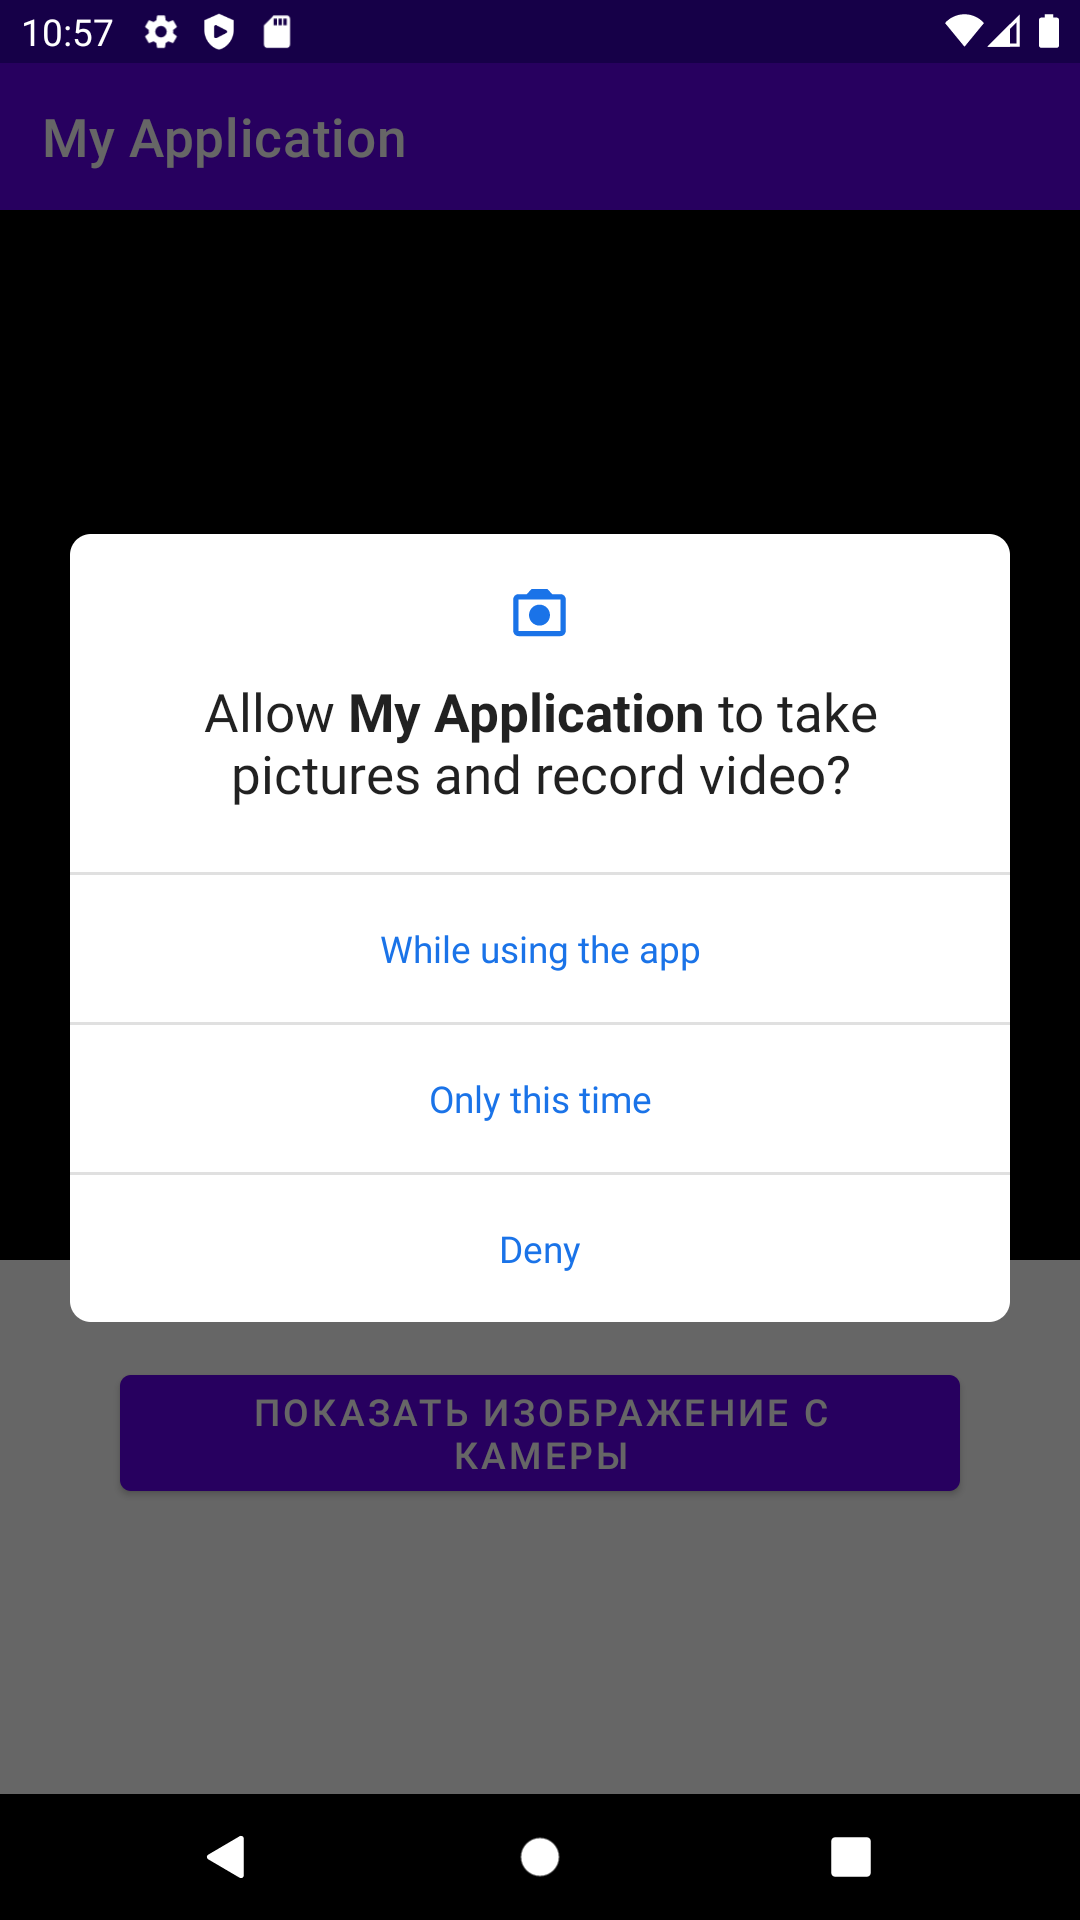
\includegraphics[width=100mm]{screen2.png}
\caption{Разрешение на использование камеры}
\label{fig:screen2}
\end{figure}

\newpage
\begin{figure}[h!]
\centering
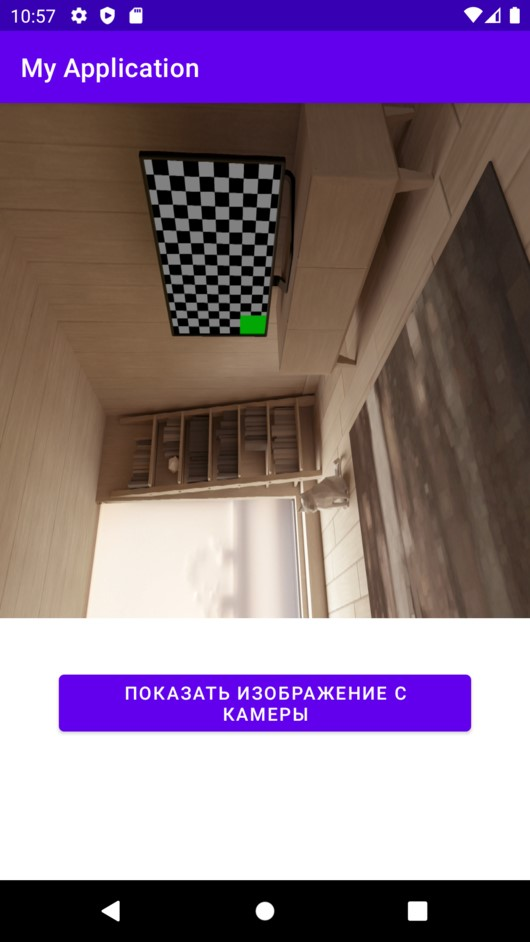
\includegraphics[width=100mm]{screen3.jpg}
\caption{Работа с камерой}
\label{fig:screen3}
\end{figure}

%%%%%%%%%%%%%%%%%%%%%%%%%%%%%%%%%%%%%%%%%%%%%%%%%%%%%%%%%%%%%%%%%%%%
\newpage
\subsection{Дизайн приложения}
Для того чтобы создать дизайн приложения, я решил использовать Flutter это набор инструментов для разработки программного обеспечения от Google для создания кроссплатформенных приложений. Так как у меня уже есть хорошие базовые знания по Flutter, я решил сделать дизайн именно в нем, чтобы улучшить свои навыки во Flutter, а также, чтобы  в будущем мне было легче сделать дизайн нашего приложение на языке Java. 
\image{flutter.png}{Официальный сайт Flutter}

\newpage
1)Экран авторизации. На экране авторизации пользователь сможет ввести логин и пароль, чтобы войти в приложение. Если он ввёл верные данные, то перейдёт на главный экран, иначе нет. Также если пользователь не зарегистрирован, то здесь он может перейти на экран регистрации.

\begin{figure}[h!]
\centering
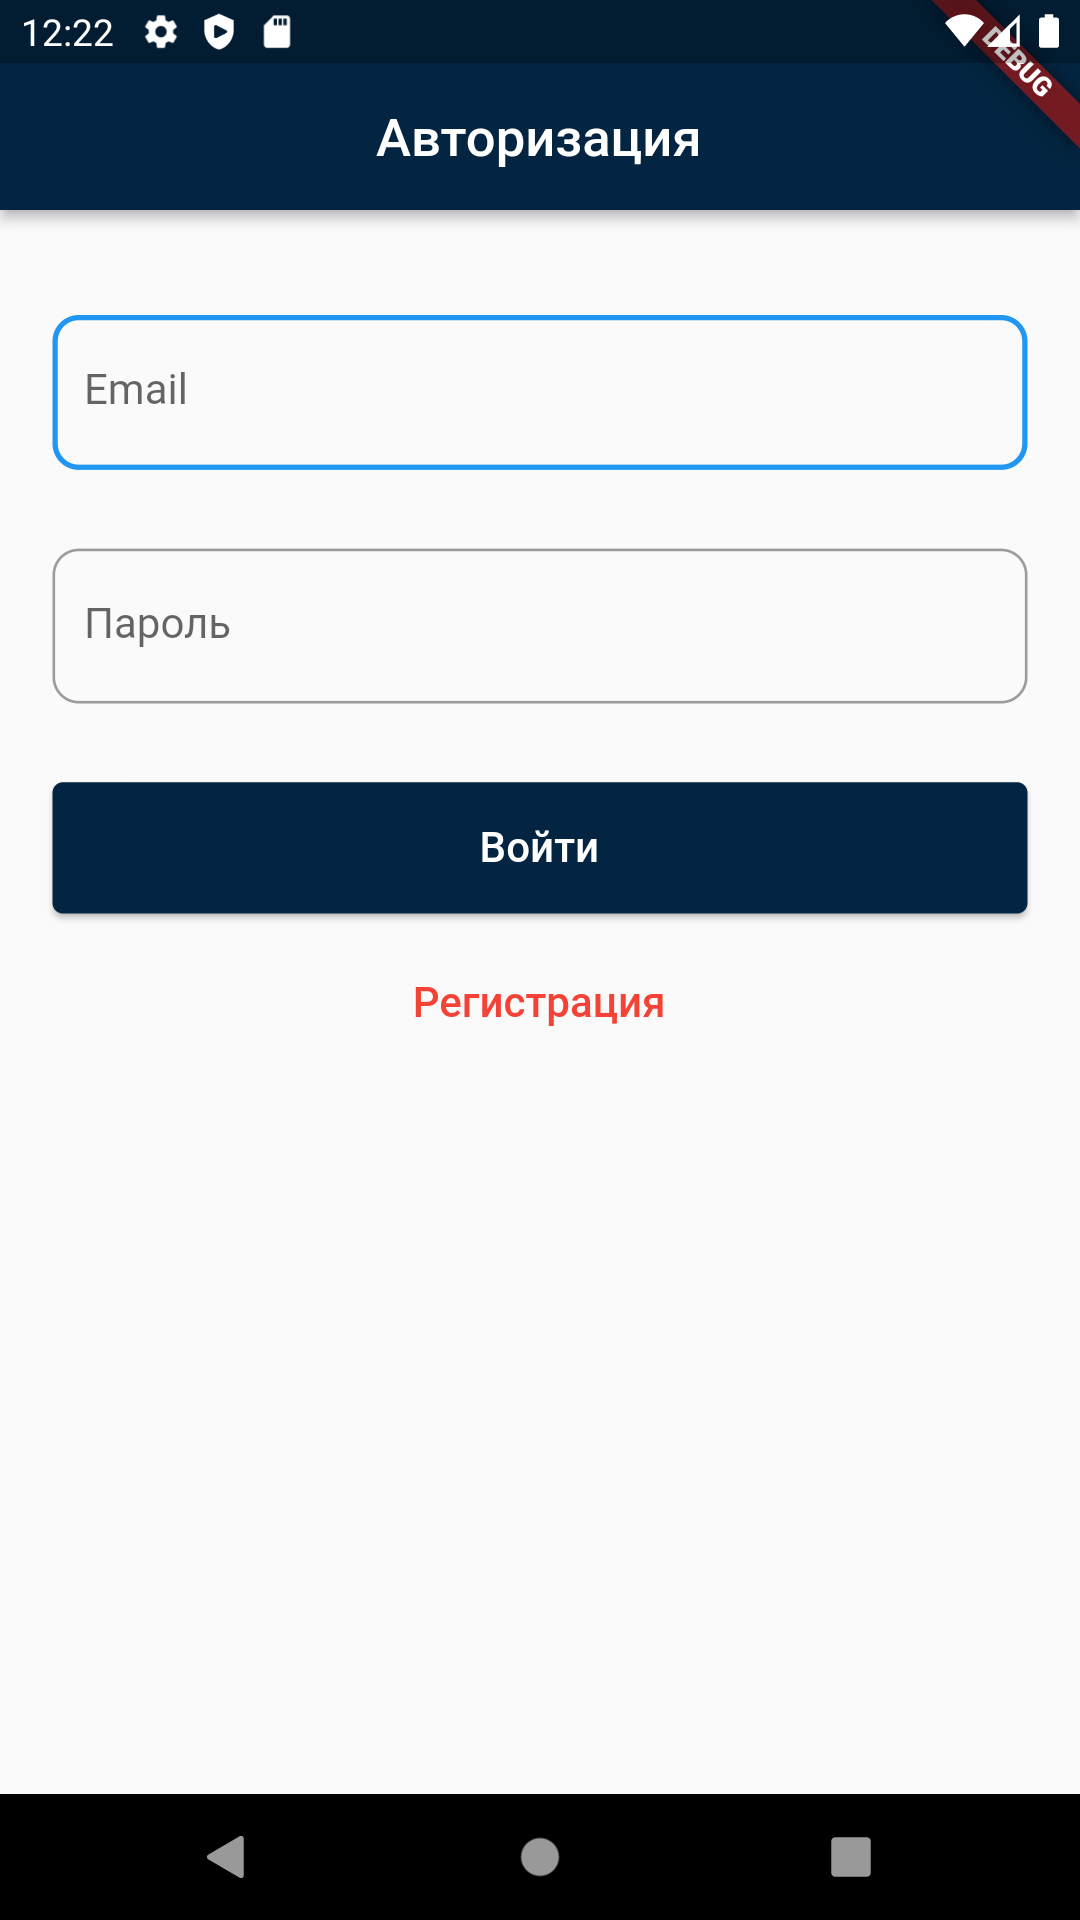
\includegraphics[width=100mm]{auth.png}
\caption{Экран авторизации}
\label{fig:auth}
\end{figure}
\newpage
2)Экран регистрации. На экране регистрации, пользователь сможет зарегистрироваться в нашем приложение, после чего перейдет на главный экран приложения.
\begin{figure}[h!]
\centering
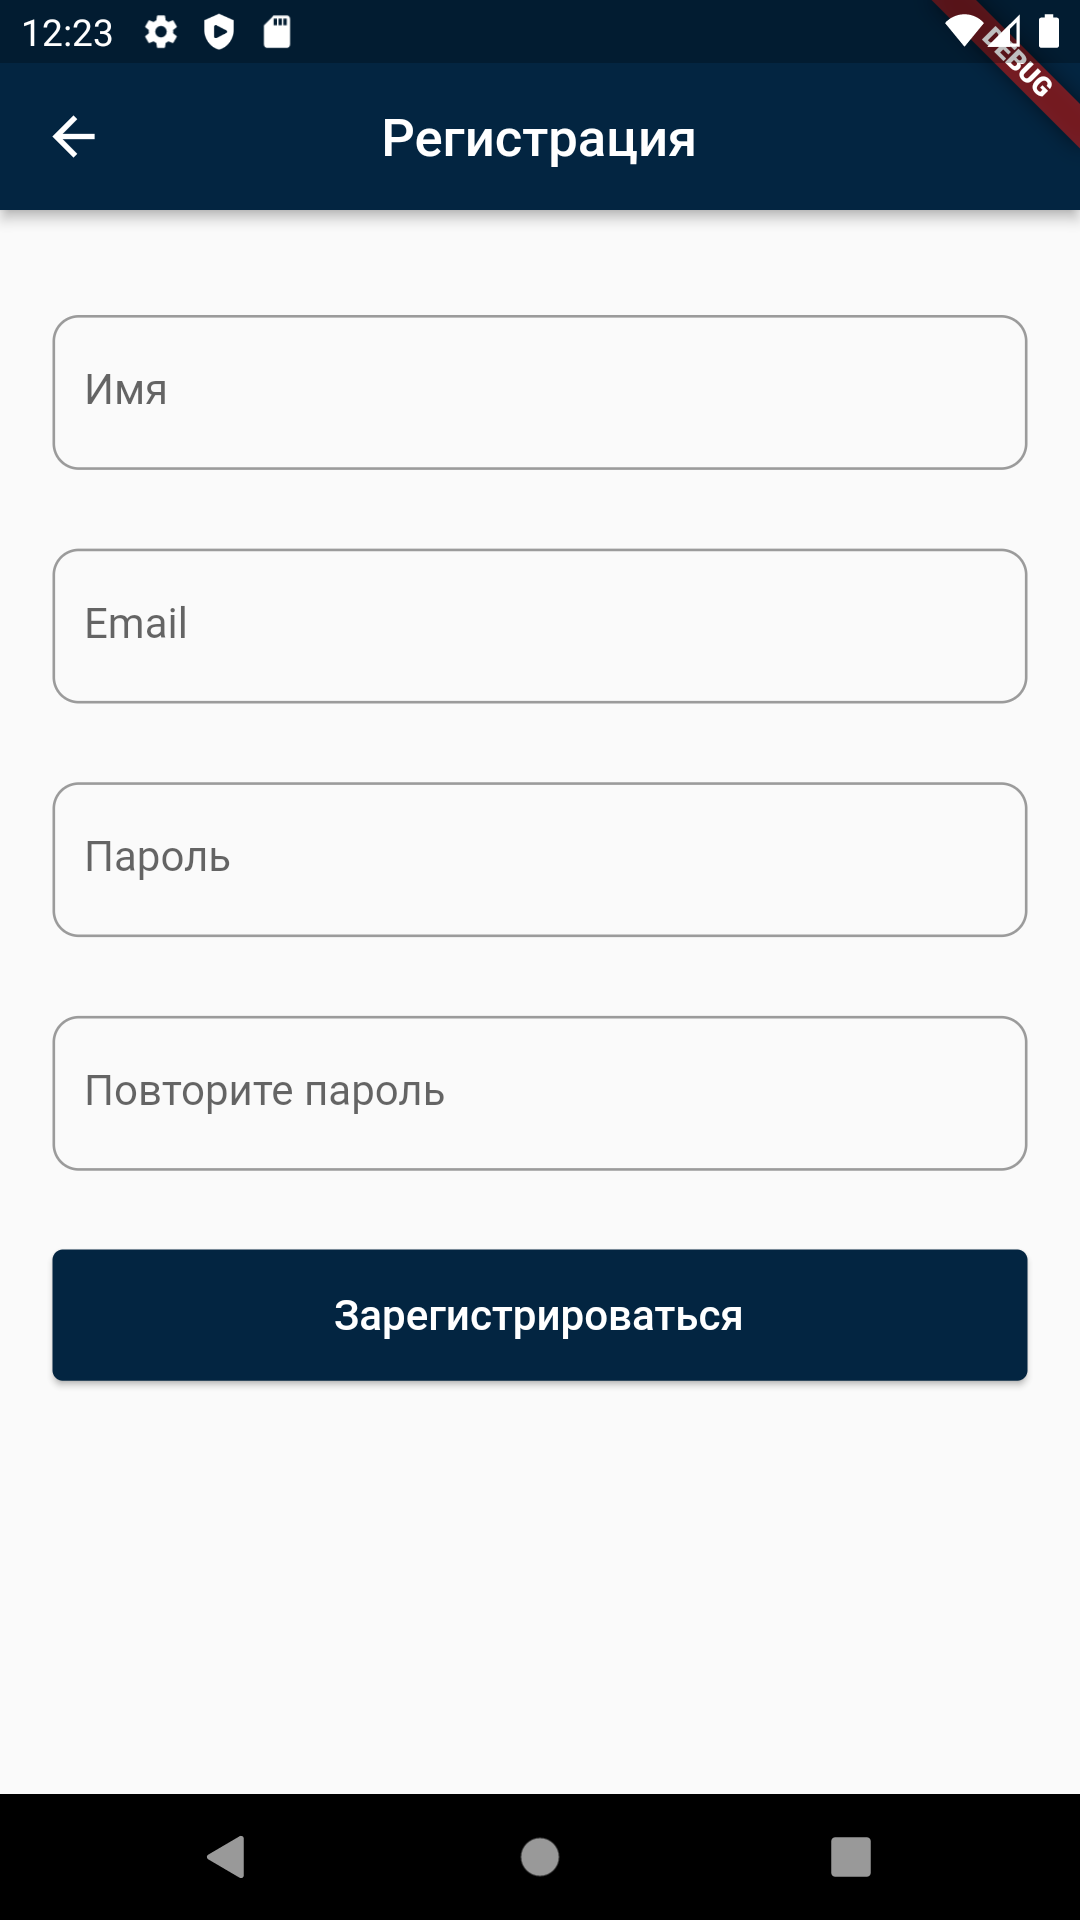
\includegraphics[width=100mm]{reg.png}
\caption{Экран регистрации}
\label{fig:reg}
\end{figure}
\newpage
3)Главный экран. На главный экран пользователь перейдет, когда он авторизуется или зарегистрируется. На главном экране находится нижняя панель навигации. Здесь пользователь сможет переходить на экран профиля и на главный экран, который стоит по умолчанию. Помимо нижнего панеля навигации пользователь сможет искать фильмы и смотреть список топ и популярных фильмов. Также если пользователь нажмет на какой либо фильм, то перейдет на экран с описанием фильма.
\begin{figure}[h!]
\centering
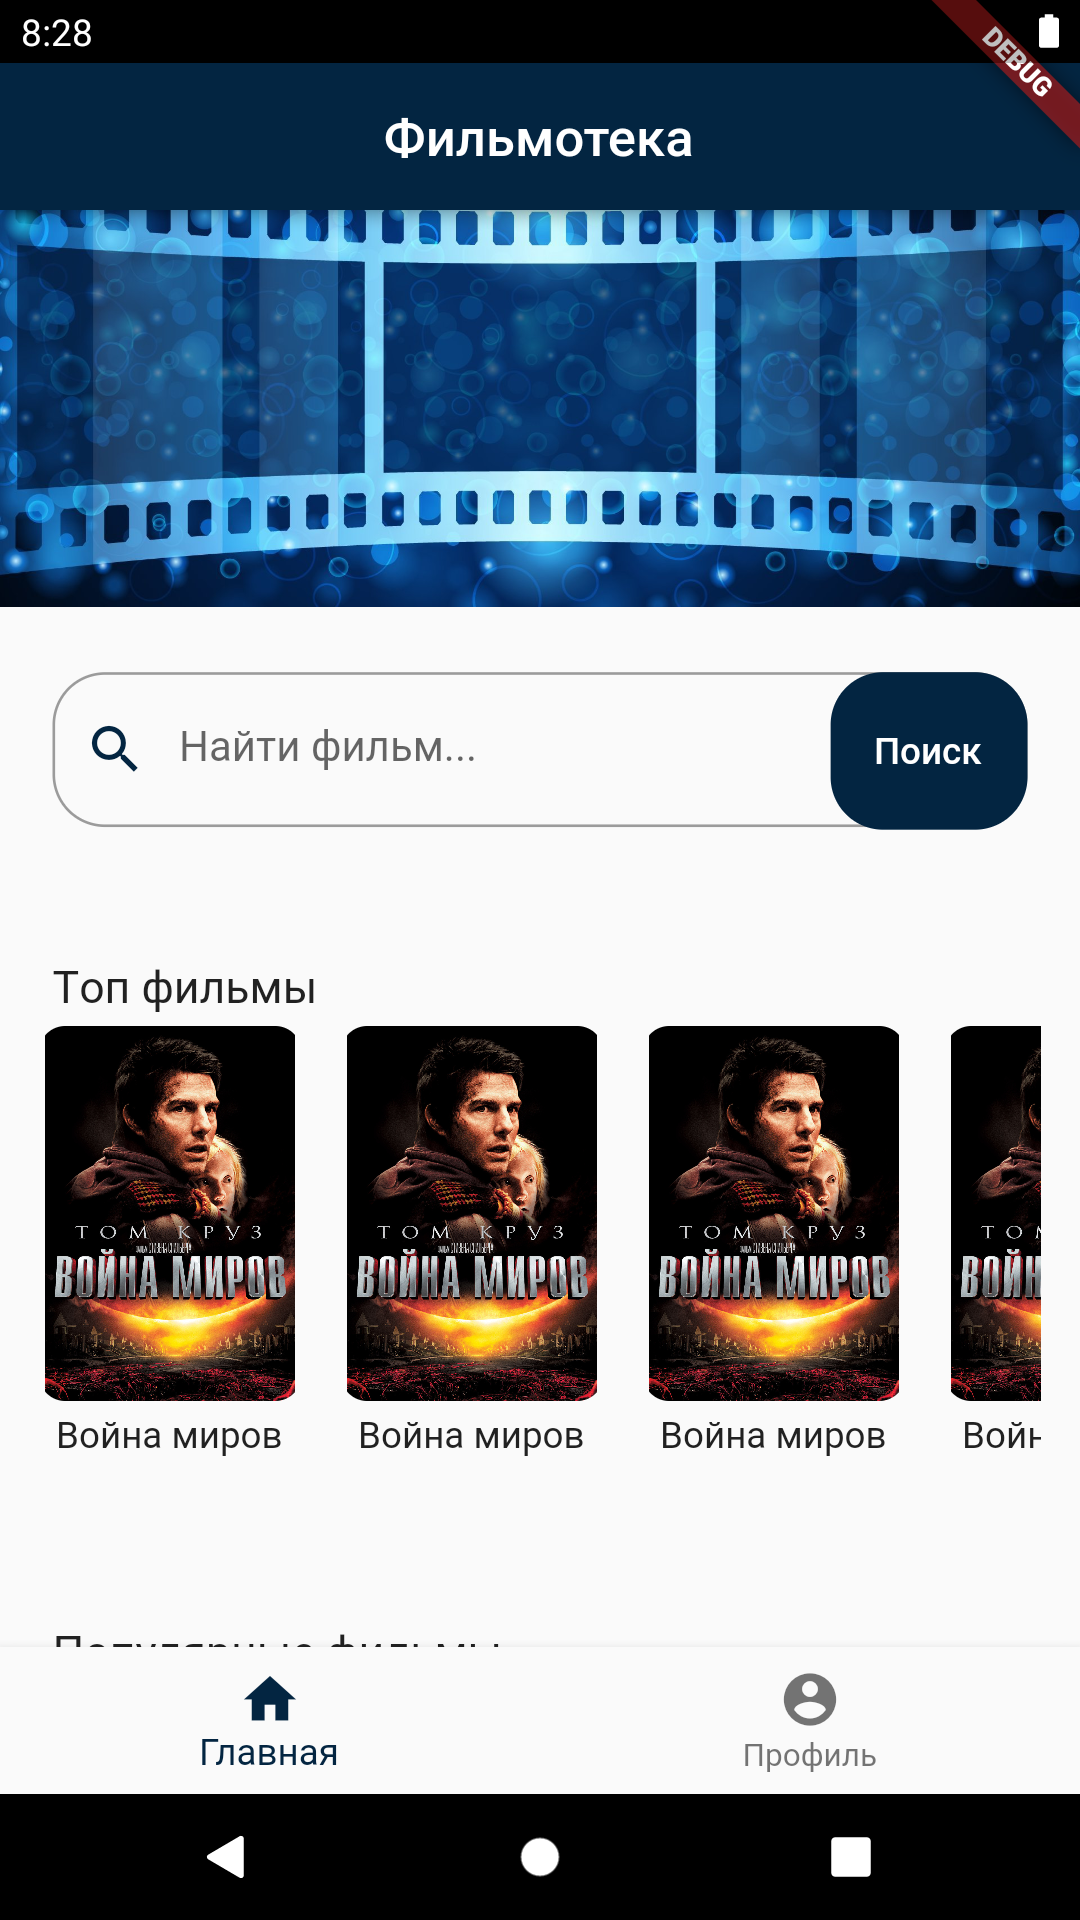
\includegraphics[width=100mm]{main.png}
\caption{Главный экран}
\label{fig:main}
\end{figure}
\newpage
4)Экран с описанием фильма. На экране с описанием фильма будет описание фильма (дата выхода, название и тд).
\begin{figure}[h!]
\centering
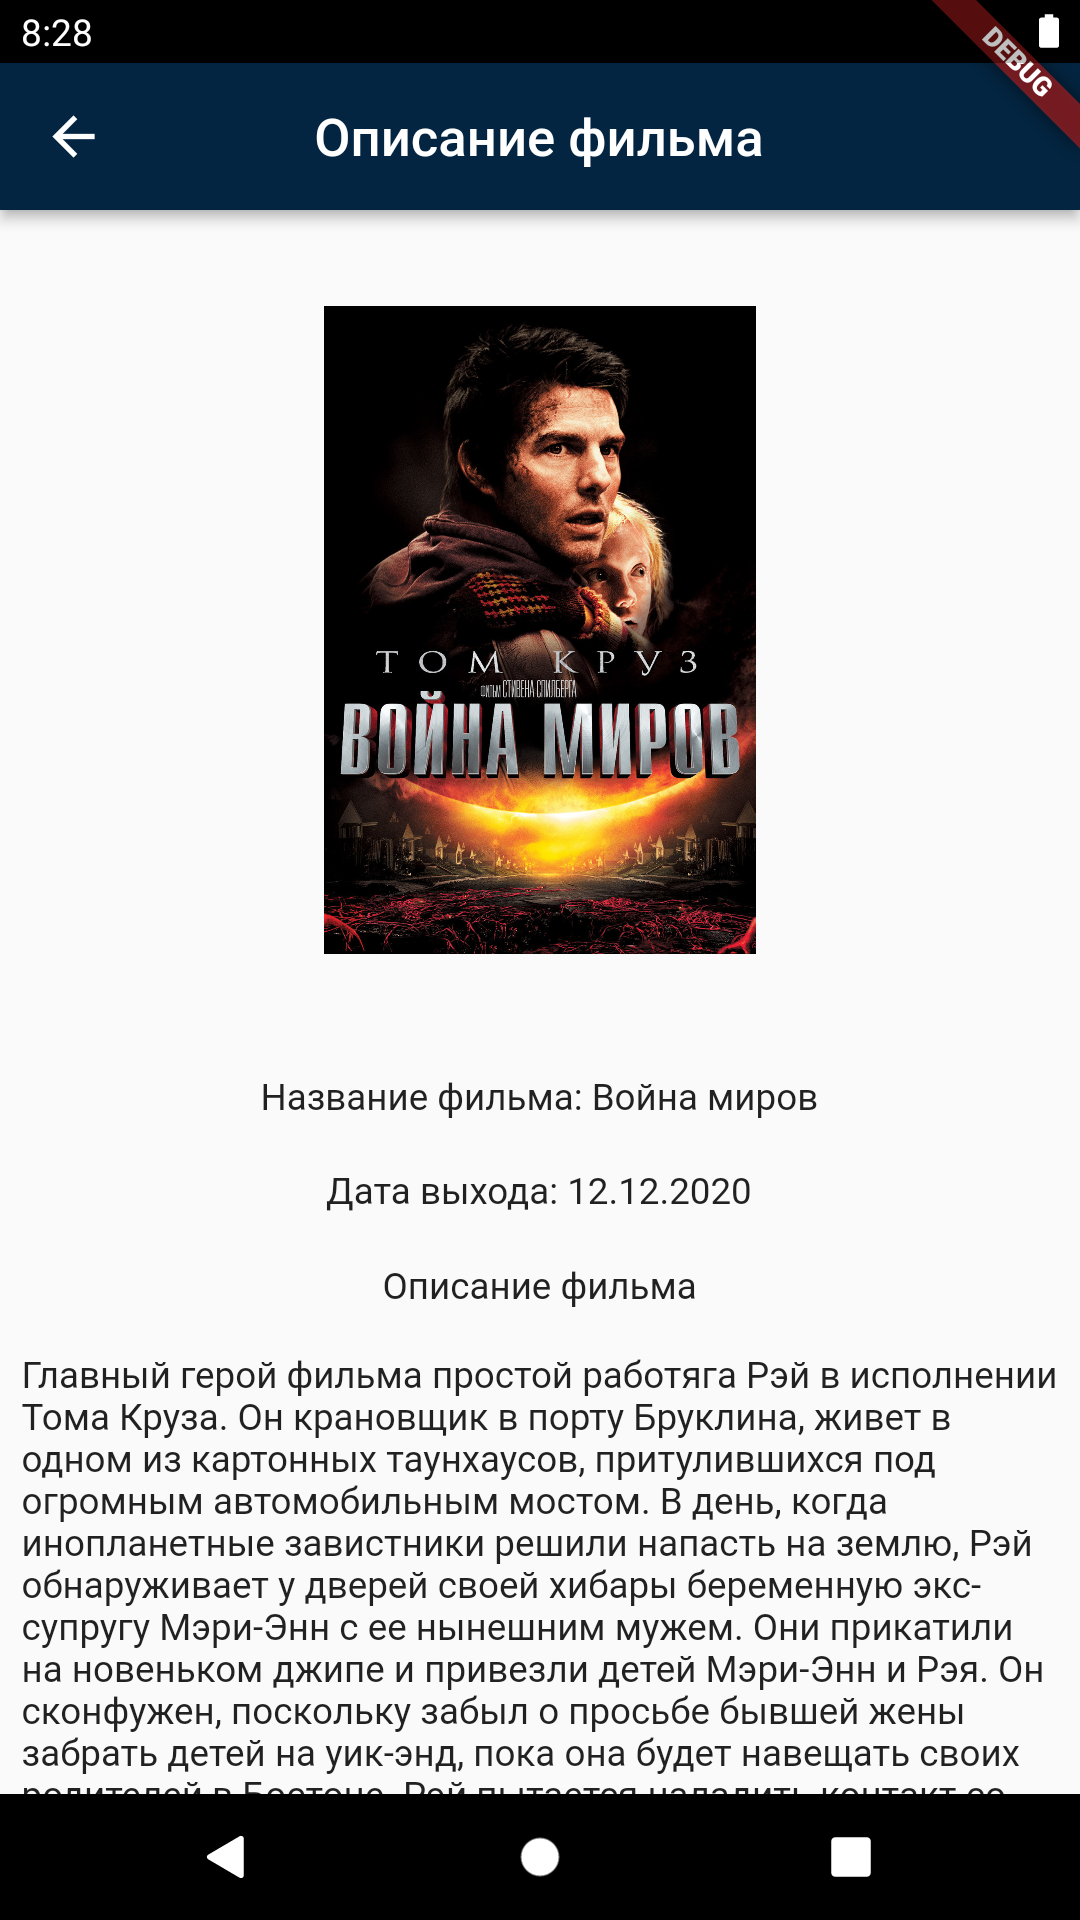
\includegraphics[width=100mm]{overview.png}
\caption{Экран c описанием фильма}
\label{fig:overview}
\end{figure}

\newpage
5)Экран с результом поиска. Экран с результатом поиска появляется когда пользователь использует поиск, который находится на главном экране. Здесь появляются фильмы, название которых идентичны или схожи с тем что ввел пользователь.
\begin{figure}[h!]
\centering
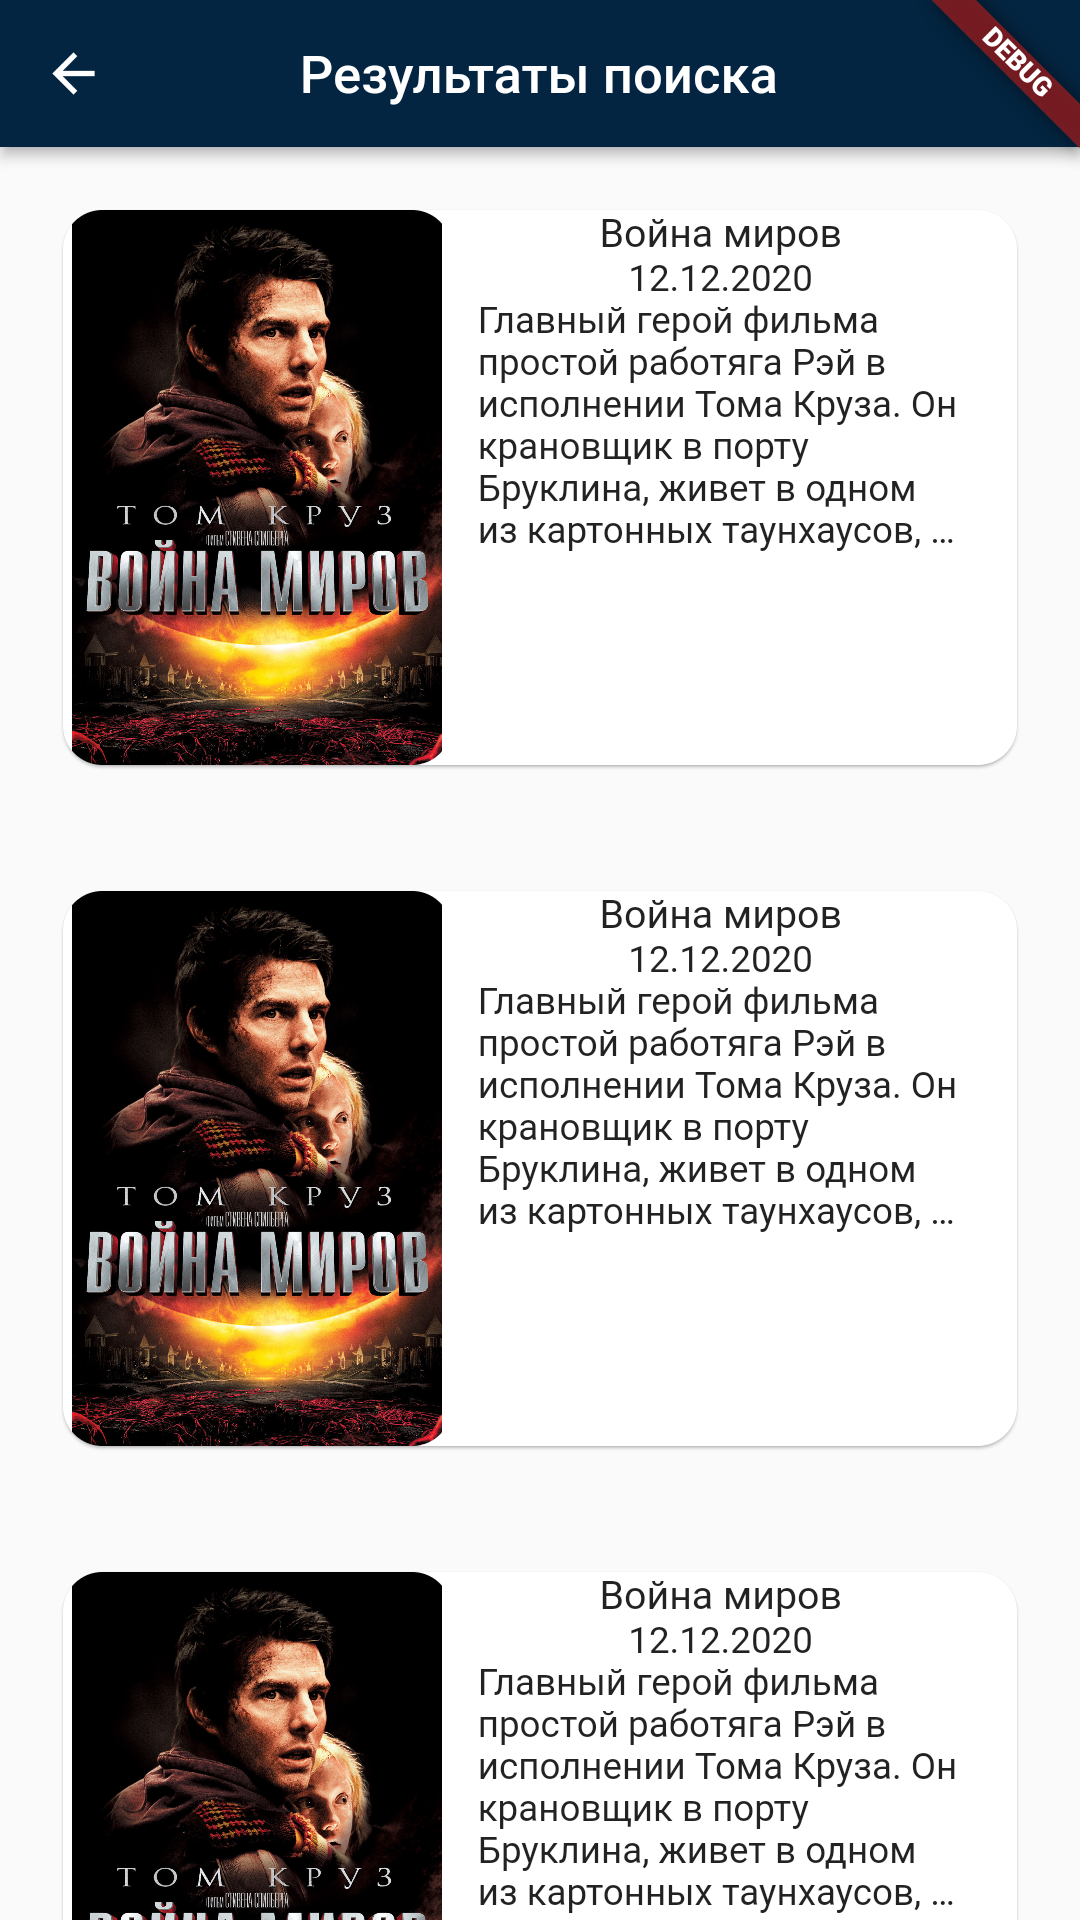
\includegraphics[width=100mm]{search_result.png}
\caption{Экран профиля}
\label{fig:profile}
\end{figure}

\newpage
6)Экран профиля. На экране профиля пользователь сможет увидеть данные об аккаунте, сменить фотографию профиля и выйти из аккаунта.
\begin{figure}[h!]
\centering
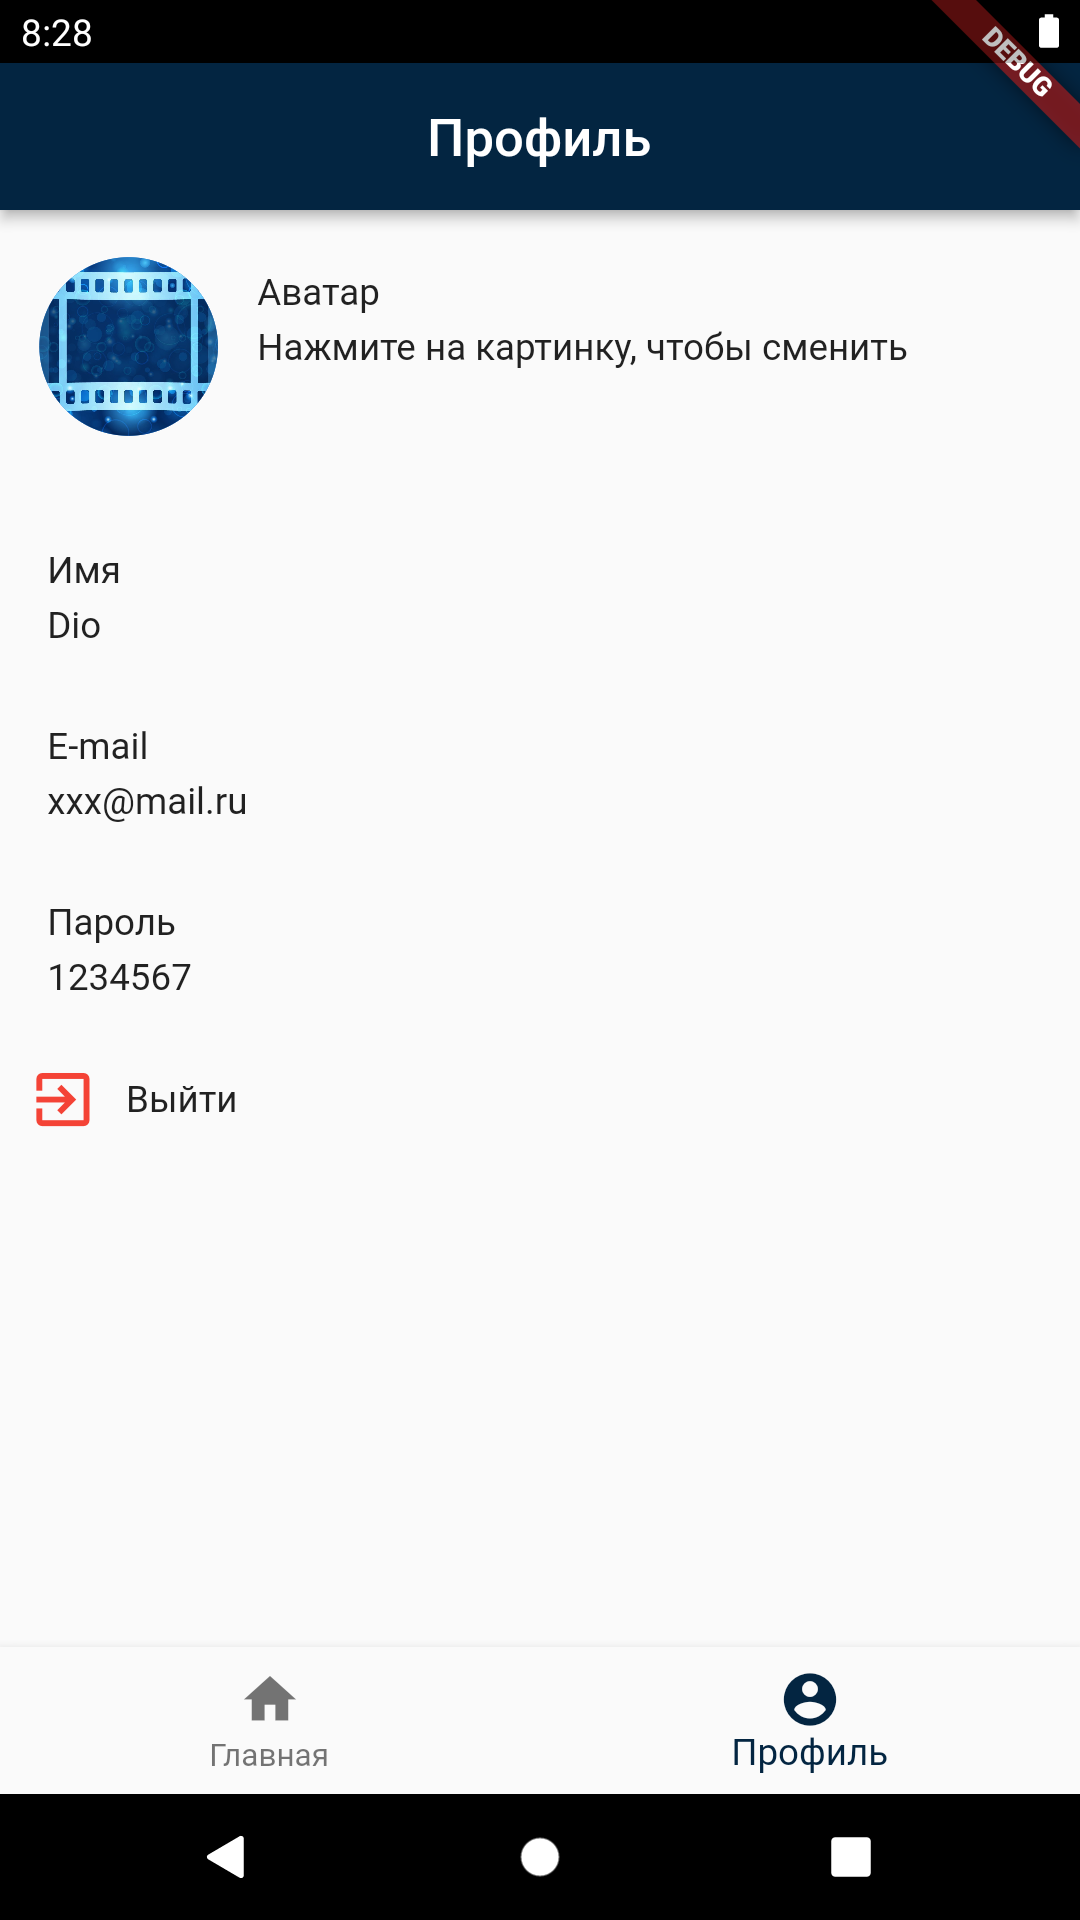
\includegraphics[width=100mm]{profile.png}
\caption{Экран профиля}
\label{fig:profile}
\end{figure}
%%%%%%%%%%%%%%%%%%%%%%%%%%%%%%%%%%%%%%%%%%%%%%%%%%%%%%%%%%%%%%%%%%%%
\newpage
\begin{center}
\section*{Заключение}
\addcontentsline{toc}{section}{Заключение}
\end{center}
В ходе выполнения курсовой работы я укрепил свои знания полученные на практических и лекционных занятиях по архитектуре мобильных\newline устройств и операционных систем. А именно работа с терминалом Linux, с\newline AndroidManifest.xml файлом, а также созданием виртуальных машин в\newline VirtualBox.
\begin{enumerate}
\item Собрал ядро OC Linux с помощъю автоматического режима.
\item Подключил модули для работы с камерой и протестировал. 
\item Создал дизайн для своего будущего приложения на тему информационно-справочная система «Фильмотека домашняя», использовав кроссплатформенный язык для разработки мобильных приложений - Flutter.
\item Составил отчет по данной курсовой работе.
\end{enumerate}
Что значит, что все требования указанные в данной курсовой работе выпонлнены, поэтому можно считать курсовую работу завершенной успешно.

%%%%%%%%%%%%%%%%%%%%%%%%%%%%%%%%%%%%%%%%%%%%%%%%%%%%%%%%%%%%%%%%%%%%
\newpage
\begin{center}
\section*{Источники}
\addcontentsline{toc}{section}{Источники}
\end{center}
\begin{enumerate}
\item Сборка ядра Linux - https://losst.ru/sobiraem-yadro-linux
\item Что такое ядро Linux - https://losst.ru/chto-takoe-yadro-linux
\item Методические указания по курсовому проектированию Архитектура операционных систем мобильных устройств 2021
\end{enumerate}

